% =========================================================================
%  Carrusel de Instagram (4:5, 1080x1350 px) con lo esencial del Tema 4.
%  Compilación: latexmk carrusel.tex ; PNG: ./exportar.sh
%  Reutiliza estilos, datos e imagen de portada de ../tema4_latex.
% =========================================================================
\documentclass[11pt]{article}
\usepackage[paperwidth=108mm, paperheight=135mm, margin=0pt]{geometry}
% Preámbulo común del carrusel y de la historia (estilo de los apuntes)
\usepackage{fontspec}
\usepackage[spanish,es-noshorthands]{babel}
\usepackage{microtype}
\usepackage{amsmath, amssymb, mathtools, bm}
\usepackage{xcolor}
\definecolor{fondo}{HTML}{000000}
\definecolor{texto}{HTML}{ECECEC}
\definecolor{blanco}{HTML}{FFFFFF}
\definecolor{negro}{HTML}{000000}
\definecolor{gris}{HTML}{9CA0A8}
\definecolor{grismedio}{HTML}{5B5F67}
\definecolor{grisoscuro}{HTML}{2E3036}
\definecolor{cajafondo}{HTML}{0E1014}
\definecolor{cian}{HTML}{20B4CE}
\definecolor{cianclaro}{HTML}{7FDBEA}
\definecolor{violeta}{HTML}{A48BFA}
\definecolor{ambar}{HTML}{F4B740}
\definecolor{magenta}{HTML}{E5579D}
\definecolor{verde}{HTML}{4FD68A}
\definecolor{naranja}{HTML}{FA8F45}
\definecolor{rojo}{HTML}{F25F5C}
\pagecolor{fondo}\color{texto}
\usepackage{graphicx}
\usepackage{tikz}
\usetikzlibrary{arrows.meta, calc, positioning}
\usepackage{pgfplots}
\pgfplotsset{compat=1.18}
\usepgfplotslibrary{fillbetween}
% =========================================================================
%  Estilos gráficos comunes (TikZ / pgfplots) para fondo negro
% =========================================================================

% --- Mapa de colores «arcoíris» para coloreado por fase (dominio complejo) ---
% Recorre el círculo cromático completo: el color codifica arg f(z) en (-pi,pi].
\pgfplotsset{colormap={fase}{
  rgb255=(255,40,60) rgb255=(255,150,20) rgb255=(250,230,40)
  rgb255=(60,220,90) rgb255=(30,200,230) rgb255=(60,90,255)
  rgb255=(190,60,240) rgb255=(255,40,60)}}

% --- Estilos TikZ generales ------------------------------------------------
\tikzset{
  >=Stealth,
  every picture/.append style={line cap=round, line join=round},
  eje/.style={-{Stealth[length=5pt,width=4pt]}, line width=0.6pt, gris},
  ejeclaro/.style={-{Stealth[length=5pt,width=4pt]}, line width=0.7pt, texto},
  fino/.style={line width=0.4pt, grismedio},
  guia/.style={densely dashed, line width=0.45pt, grismedio},
  punteado/.style={densely dotted, line width=0.6pt, gris},
  etiq/.style={font=\small, text=texto},
  etiqgris/.style={font=\footnotesize, text=gris},
  polo/.style={cross out, draw=rojo, line width=1.1pt, minimum size=6pt, inner sep=0pt},
  punto/.style={circle, fill=blanco, inner sep=0pt, minimum size=4pt},
  puntocian/.style={circle, fill=cian, inner sep=0pt, minimum size=4.5pt},
  orienta/.style={decoration={markings, mark=at position #1 with
     {\arrow{Stealth[length=6pt,width=5pt]}}}, postaction={decorate}},
  orienta/.default=0.55,
  nodo/.style={draw=grismedio, fill=cajafondo, rounded corners=2pt,
     line width=0.5pt, inner xsep=6pt, inner ysep=4pt, font=\small, text=texto},
  nodocian/.style={nodo, draw=cian},
  nodoambar/.style={nodo, draw=ambar},
  nodovioleta/.style={nodo, draw=violeta},
  flecha/.style={-{Stealth[length=5pt,width=4.5pt]}, line width=0.6pt, gris},
}

% --- Estilo base de ejes pgfplots en oscuro ----------------------------------
\pgfplotsset{
  oscuro/.style={
    axis background/.style={fill=fondo},
    tick label style={font=\scriptsize, text=gris},
    label style={font=\small, text=texto},
    title style={font=\small, text=texto},
    axis line style={grismedio, line width=0.5pt},
    every tick/.style={grismedio},
    major tick length=3pt,
    grid=major, grid style={grisoscuro, line width=0.35pt},
    legend style={font=\scriptsize, draw=grisoscuro, fill=cajafondo,
                  text=texto, rounded corners=1.5pt, inner sep=3pt,
                  row sep=1pt},
    legend cell align=left,
    /pgf/number format/use comma,
    /pgf/number format/1000 sep={},
    unbounded coords=jump,
  },
  % Ejes cruzados por el origen (estilo «pizarra»)
  cruz/.style={oscuro, axis lines=middle, grid=none,
    axis line style={gris, line width=0.6pt,
      -{Stealth[length=5pt,width=4pt]}},
    xlabel style={anchor=west, font=\small},
    ylabel style={anchor=south, font=\small},
  },
  superficie/.style={
    tick label style={font=\scriptsize, text=gris},
    label style={font=\small, text=texto},
    axis line style={grismedio}, every tick/.style={grismedio},
    grid=none, colormap name=fase, shader=interp,
    /pgf/number format/use comma,
  },
  % Curvas
  c1/.style={line width=1.15pt, cian},
  c2/.style={line width=1.15pt, magenta},
  c3/.style={line width=1.15pt, ambar},
  c4/.style={line width=1.15pt, verde},
  c5/.style={line width=1.15pt, violeta},
  c6/.style={line width=1.15pt, naranja},
}


% Escala progresiva para familias de curvas (azul -> violeta)
\definecolor{cm1}{RGB}{60,90,255}
\definecolor{cm2}{RGB}{45,145,240}
\definecolor{cm3}{RGB}{30,200,230}
\definecolor{cm4}{RGB}{60,220,90}
\definecolor{cm5}{RGB}{250,230,40}
\definecolor{cm6}{RGB}{255,150,20}
\definecolor{cm7}{RGB}{255,40,60}
\definecolor{cm8}{RGB}{190,60,240}

\pagestyle{empty}
\setlength{\parindent}{0pt}

\DeclareMathOperator{\sen}{sen}
\renewcommand{\sin}{\sen}
\newcommand{\Lop}{\mathcal{L}}
\newcommand{\dif}{\mathrm{d}}
\newcommand{\eul}{\mathrm{e}}
\newcommand{\T}{\mathsf{T}}
\newcommand{\yv}{\hat{\bm y}}
\newcommand{\ubr}[2]{\underbrace{#1}_{\textcolor{gris}{#2}}}
\newcommand{\R}{\mathbb{R}}

% Caja con pestaña, en el estilo de los apuntes
\tikzset{caja/.style={draw=#1, fill=cajafondo, rounded corners=2.5pt,
    line width=0.7pt, inner xsep=8pt, inner ysep=7pt, text width=8.6cm,
    align=flush center, text=texto},
  pestana/.style={fill=#1, rounded corners=2pt, inner xsep=5pt, inner ysep=1.6pt,
    font=\sffamily\bfseries\scriptsize, text=negro},
  chip/.style={draw=#1, fill=cajafondo, rounded corners=2.5pt, line width=0.7pt,
    inner xsep=6pt, inner ysep=6pt, minimum width=4.3cm, minimum height=1.05cm,
    align=flush center, text=texto}}



\newcommand{\total}{7}
% Marco común: cabecera, título y paginación por puntos
% #1 número, #2 rótulo pequeño, #3 título
\newcommand{\marco}[3]{%
  \node[anchor=west, inner sep=0] at (0.8,12.85)
    {\color{gris}\scshape\scriptsize\textls[120]{Ecuaciones Diferenciales\ ·\ Tema 4}};
  \node[anchor=east, inner sep=0] at (10.0,12.85)
    {\color{cian}\sffamily\bfseries\scriptsize #1\,/\,\total};
  \draw[grisoscuro, line width=0.4pt] (0.8,12.55) -- (10.0,12.55);
  \ifx\relax#2\relax\else
  \node[anchor=west, inner sep=0] at (0.8,12.0)
    {\color{cian}\sffamily\bfseries\footnotesize\textls[80]{#2}};
  \node[anchor=north west, inner sep=0, text width=9.2cm] at (0.8,11.7)
    {\color{blanco}\bfseries\Large #3};
  \fi
  \foreach \k in {1,...,\total}{
    \ifnum\k=#1\relax
      \fill[cian] ({5.4+(\k-4)*0.32},0.6) circle (0.075);
    \else
      \fill[grismedio] ({5.4+(\k-4)*0.32},0.6) circle (0.05);
    \fi}
}
\newcommand{\lienzo}{\useasboundingbox (0,0) rectangle (10.8,13.5);}
\newenvironment{diapo}{\noindent\begin{tikzpicture}\lienzo}{\end{tikzpicture}\newpage}
\begin{document}

% =================================================================== 1
\begin{diapo}
  \marco{1}{}{}
  \node[anchor=north, align=flush center, text width=10cm, inner sep=0] at (5.4,12.2)
    {{\color{cian}\scshape\footnotesize\textls[200]{Tema 4}}\\[6pt]
     {\color{blanco}\fontsize{25}{29}\selectfont\bfseries EDO lineales\\de orden superior}\\[7pt]
     {\color{cian}\rule{2.4cm}{0.6pt}}\\[5pt]
     {\color{texto}\itshape\small de la linealidad a la función de Green}};
  \node[inner sep=0] at (5.4,5.95)
    {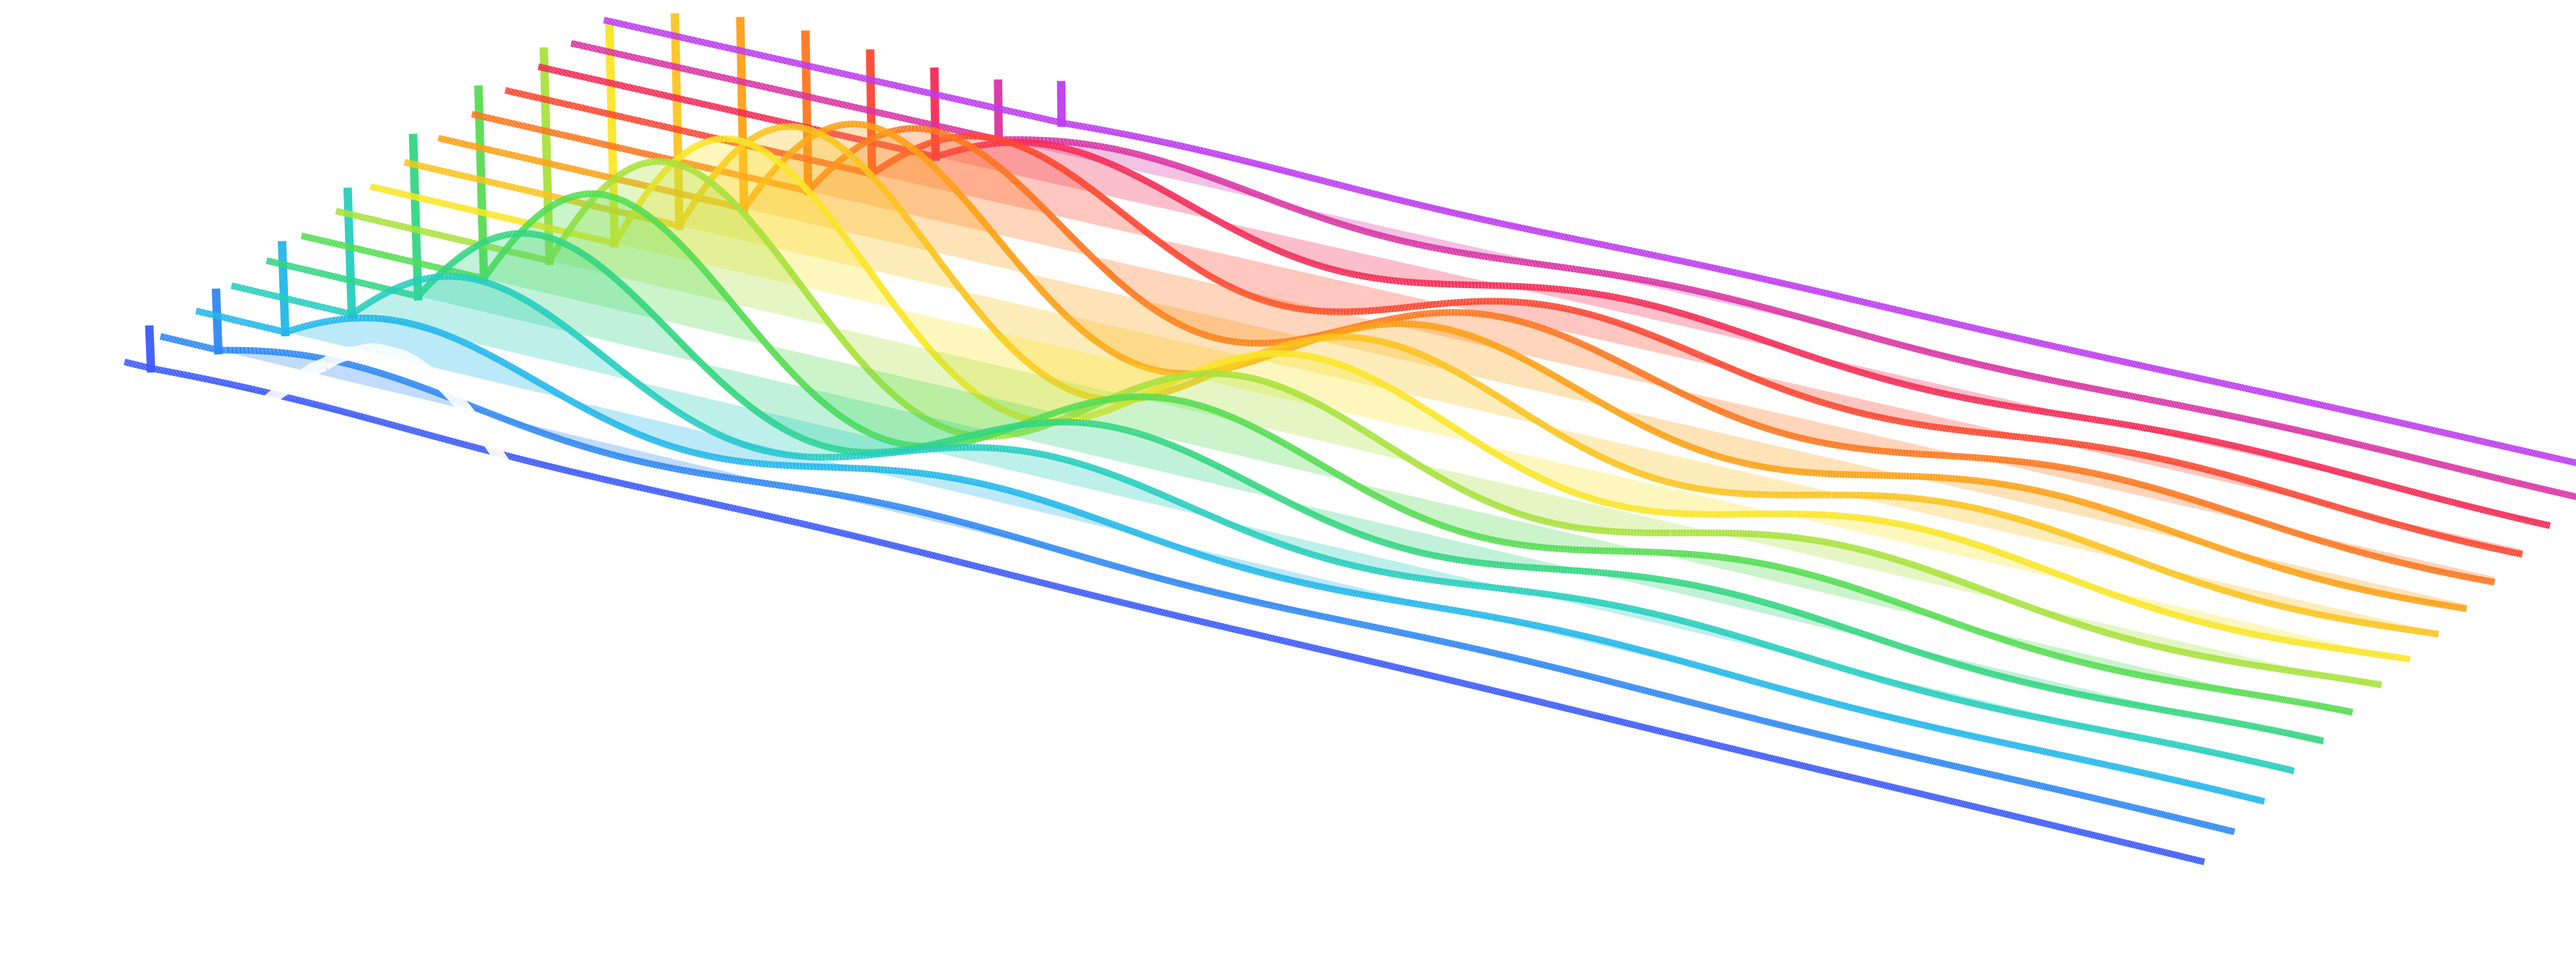
\includegraphics[width=11.6cm]{../tema4_latex/figuras/portada_superficie.png}};
  \node[chip=cian]    at (3.05,2.95) {$\displaystyle\Lop=\sum_{j=0}^{n}a_j(x)\,D^{j}$};
  \node[chip=violeta] at (7.75,2.95) {$\dim\ker\Lop=n$};
  \node[chip=ambar]   at (3.05,1.7) {$W(x)\,\bm k'(x)=\bm b(x)$};
  \node[chip=magenta] at (7.75,1.7) {$\Lop_xG(x,\tilde x)=\delta(x-\tilde x)$};
  \node[anchor=east, inner sep=0] at (10.0,0.6)
    {\color{gris}\itshape\scriptsize desliza $\longrightarrow$};
\end{diapo}

% =================================================================== 2
\begin{diapo}
  \marco{2}{01 · ESTRUCTURA}{Todo descansa en la linealidad}
  \node[anchor=north, align=flush center, text width=9.2cm, inner sep=0] at (5.4,10.75)
    {$\Lop[y]=a_n(x)\,y^{(n)}+\dots+a_1(x)\,y'+a_0(x)\,y=b(x)$\\[8pt]
     $\Lop[\alpha y_1+\beta y_2]=\alpha\,\Lop[y_1]+\beta\,\Lop[y_2]$};
  \node[caja=violeta] (t) at (5.4,7.85)
    {$\Phi_{x_0}\colon\ker\Lop\xrightarrow{\ \cong\ }\R^{n},\quad
      y\longmapsto\begin{pmatrix}y(x_0)\\[-2pt] \vdots\\ y^{(n-1)}(x_0)\end{pmatrix}$\\[5pt]
     {\small existencia $\Rightarrow$ sobre $\cdot$ unicidad $\Rightarrow$ inyectiva}};
  \node[pestana=violeta, anchor=west] at ($(t.north west)+(0.3,0)$) {Dimensión del núcleo};
  \begin{axis}[oscuro, at={(1.2cm,3.35cm)}, anchor=south west, width=9.3cm, height=3.7cm,
      xmin=-0.3, xmax=6.6, ymin=-1.6, ymax=1.75, xtick={0,3.14159,6.28318},
      xticklabels={$0$,$\pi$,$2\pi$}, ytick={-1,0,1}, samples=200, domain=-0.3:6.6,
      title={\footnotesize $y''+y=0$: cada par de datos, una única curva}]
    \addplot[c1] {cos(deg(x))};
    \addplot[c2] {sin(deg(x))};
    \addplot[c3] {cos(deg(x))+sin(deg(x))};
    \addplot[c4] {-0.5*cos(deg(x))+0.8*sin(deg(x))};
    \addplot[only marks, mark=*, mark size=1.7pt, blanco] coordinates {(0,1) (0,0) (0,-0.5)};
  \end{axis}
  \node[anchor=north, inner sep=0] at (5.4,2.75)
    {$y=\ubr{\sum_{i=1}^{n}c_i\,\hat y_i}{y_h\,\in\,\ker\Lop}+\;\ubr{y_p}{\text{particular}}$};
\end{diapo}

% =================================================================== 3
\begin{diapo}
  \marco{3}{02 · WRONSKIANO}{Independencia y Abel--Liouville}
  \node[anchor=north, align=flush center, text width=9.4cm, inner sep=0] at (5.4,10.95)
    {$W=\begin{pmatrix}\hat y_1 & \cdots & \hat y_n\\ \vdots & & \vdots\\
      \hat y_1^{(n-1)} & \cdots & \hat y_n^{(n-1)}\end{pmatrix},\qquad
      w=\det W$\\[6pt]
     $W(x_0)\,\bm c=\Phi_{x_0}\bigl(\textstyle\sum_i c_i\hat y_i\bigr)$\\[6pt]
     {\small base de $\ker\Lop$ $\iff$ $w(x_0)\neq0$ $\iff$ $w(x)\neq0\ \ \forall x\in I$}};
  \node[caja=ambar] (a) at (5.4,6.5)
    {$\displaystyle w(x)=w(x_0)\,\exp\!\Bigl(-\int_{x_0}^{x}\frac{a_{n-1}(s)}{a_n(s)}\,\dif s\Bigr)$\\[3pt]
     {\small $w$ nunca se anula, o es idénticamente nulo}};
  \node[pestana=ambar, anchor=west] at ($(a.north west)+(0.3,0)$) {Abel--Liouville};
  \begin{axis}[cruz, at={(1.3cm,1.7cm)}, anchor=south west, width=9.0cm, height=3.6cm,
      xmin=-1.6, xmax=1.6, ymin=-2.3, ymax=2.3, xtick=\empty, ytick=\empty,
      samples=200, domain=-1.5:1.5, clip=false]
    \addplot[c1] {x^2};
    \addplot[c2, densely dashed] {x*abs(x)};
    \node[font=\footnotesize, text=cian, anchor=west] at (axis cs:1.2,1.2) {$x^{2}$};
    \node[font=\footnotesize, text=magenta, anchor=west] at (axis cs:-0.95,-1.7) {$x\,\lvert x\rvert$};
    \node[font=\footnotesize, text=gris, align=left, anchor=north west] at (axis cs:0.2,-0.45)
      {independientes,\\pero $w\equiv0$};
  \end{axis}
  \node[anchor=north, inner sep=0, text width=9.2cm, align=flush center] at (5.4,1.3)
    {\color{gris}\scriptsize sin una EDO común no hay unicidad que fuerce $w\neq0$};
\end{diapo}

% =================================================================== 4
\begin{diapo}
  \marco{4}{03 · COEFICIENTES CONSTANTES}{La exponencial es autofunción}
  \node[anchor=north, align=flush center, text width=9.4cm, inner sep=0] at (5.4,10.8)
    {$\Lop=p(D),\qquad \Lop\bigl[\eul^{\lambda x}\bigr]=p(\lambda)\,\eul^{\lambda x}$\\[8pt]
     $p(\lambda)=a_n\prod_{k}(\lambda-\lambda_k)^{m_k}$\\[6pt]
     $\Longrightarrow\quad
      \ker\Lop=\bigl\langle x^{j}\eul^{\lambda_kx}\bigr\rangle_{0\le j<m_k}$};
  \begin{axis}[oscuro, at={(1.2cm,3.1cm)}, anchor=south west, width=9.3cm, height=4.6cm,
      xmin=0, xmax=14, ymin=-0.8, ymax=1.1, xtick={0,4,...,12}, ytick={-0.5,0,0.5,1},
      samples=300, domain=0:14, legend pos=north east,
      title={\footnotesize $y''+\nu\,y'+y=0$,\quad $y(0)=1$, $y'(0)=0$}]
    \addplot[c1] {exp(-0.25*x)*(cos(deg(0.968246*x))+0.258199*sin(deg(0.968246*x)))};
    \addplot[c4] {(1+x)*exp(-x)};
    \addplot[c2] {(-2.618034*exp(-0.381966*x)+0.381966*exp(-2.618034*x))/(-2.236068)};
    \legend{$\nu=0{,}5$ sub, $\nu=2$ crítico, $\nu=3$ sobre}
  \end{axis}
  \node[anchor=north, align=flush center, inner sep=0] at (5.4,2.75)
    {$\lambda_\pm=\tfrac12\bigl(-\nu\pm\sqrt{\nu^{2}-4}\bigr)$\\[6pt]
     {\color{gris}\scriptsize raíz doble en $\nu=2$: aparece $x\,\eul^{-x}$, el regreso más rápido sin oscilar}};
\end{diapo}

% =================================================================== 5
\begin{diapo}
  \marco{5}{04 · VARIACIÓN DE LAS CONSTANTES}{Promover las constantes a funciones}
  \node[anchor=north, align=flush center, text width=9.4cm, inner sep=0] at (5.4,10.8)
    {$y_p=\sum_{i}k_i(x)\,\hat y_i(x),\qquad \sum_{i}k_i'\,\hat y_i^{(j)}=0,\quad j\le n-2$\\[8pt]
     $\begin{pmatrix}\hat y_1 & \cdots & \hat y_n\\ \vdots & & \vdots\\
      \hat y_1^{(n-1)} & \cdots & \hat y_n^{(n-1)}\end{pmatrix}
      \begin{pmatrix}k_1'\\ \vdots\\ k_n'\end{pmatrix}
      =\begin{pmatrix}0\\ \vdots\\ b/a_n\end{pmatrix}$};
  \node[anchor=north, align=flush center, text width=9.4cm, inner sep=0] at (5.4,7.75)
    {{\color{gris}\scriptsize Cramer y la delta de Kronecker}\\[3pt]
     $\det A[i\!\leftarrow\!\bm u_j]=\delta_{ij}\det A$\\[4pt]
     $\Longrightarrow\quad k_i'=\dfrac{(-1)^{n+i}M_{ni}}{w}\,\dfrac{b}{a_n}$};
  \node[caja=ambar] (f) at (5.4,4.25)
    {$\displaystyle y_p(x)=\yv^{\T}(x)\int_{x_0}^{x}W^{-1}(s)\,\bm e_n\,\frac{b(s)}{a_n(s)}\,\dif s$\\[4pt]
     {\small arranca en reposo: $y_p^{(j)}(x_0)=0$}};
  \node[pestana=ambar, anchor=west] at ($(f.north west)+(0.3,0)$) {Fórmula de variación};
  \node[anchor=north, align=flush center, inner sep=0] at (5.4,2.85)
    {{\color{gris}\scriptsize oscilador forzado $y''+\omega^{2}y=b$}\\[3pt]
     $y_p(x)=\dfrac1\omega\displaystyle\int_{x_0}^{x}\sin\omega(x-s)\,b(s)\,\dif s$};
\end{diapo}

% =================================================================== 6
\begin{diapo}
  \marco{6}{05 · FUNCIÓN DE GREEN}{La respuesta a un impulso}
  \node[anchor=north, align=flush center, text width=9.4cm, inner sep=0] at (5.4,10.8)
    {$\Lop_x\,G(x,\tilde x)=\delta(x-\tilde x),\qquad
      y_p(x)=\int G(x,\tilde x)\,b(\tilde x)\,\dif\tilde x$\\[8pt]
     $\partial_x^{\,n-1}G\,\Big|_{\tilde x^-}^{\tilde x^+}=\dfrac{1}{a_n(\tilde x)}$
     \quad{\color{gris}\small (las anteriores, continuas)}};
  \begin{axis}[oscuro, at={(1.2cm,2.7cm)}, anchor=south west, width=9.3cm, height=5.6cm,
      xmin=0, xmax=20, ymin=-0.85, ymax=1.5, xtick={0,5,...,20}, ytick={-0.5,0,0.5,1},
      legend style={at={(0.985,0.97)}, anchor=north east},
      title={\footnotesize $y''+0{,}32\,y'+y=b$: $8$ impulsos y su suma}]
    \addplot[draw=none, fill=grisoscuro, forget plot] table[x=x, y=b] {../tema4_latex/datos/superposicion.dat} \closedcycle;
    \foreach \c [count=\k] in {cm1,cm2,cm3,cm4,cm5,cm6,cm7,cm8}{
      \edef\temp{\noexpand\addplot[line width=0.8pt, \c, forget plot]
        table[x=x, y=r\k] {../tema4_latex/datos/superposicion.dat};}
      \temp}
    \addplot[ambar, line width=1.1pt, densely dashed] table[x=x, y=suma] {../tema4_latex/datos/superposicion.dat};
    \addplot[blanco, line width=1.5pt] table[x=x, y=yp] {../tema4_latex/datos/superposicion.dat};
    \legend{suma, $y_p=\int G\,b$}
  \end{axis}
  \node[anchor=north, align=flush center, text width=9.4cm, inner sep=0, font=\scriptsize, text=gris] at (5.4,1.95)
    {la fuente (gris) se trocea en impulsos; cada uno da una respuesta causal\\
     y su superposición tiende a $y_p$ cuando $\Delta\tilde x\to0$};
\end{diapo}

% =================================================================== 7
\begin{diapo}
  \marco{7}{EN UNA LÍNEA}{Datos iniciales + fuente}
  \node[anchor=north, align=flush center, text width=9.6cm, inner sep=0] at (5.4,10.6)
    {$\displaystyle y(x)=\ubr{\sum_{i=1}^{n}c_i\,\hat y_i(x)}{\text{datos iniciales}}
      \;+\;\ubr{\int_{x_0}^{x}G(x,s)\,b(s)\,\dif s}{\text{fuente}}$};
  \node[caja=magenta] (g) at (5.4,7.75)
    {$G(x,s)=\Theta(x-s)\;\yv^{\T}(x)\,W^{-1}(s)\,\dfrac{\bm e_n}{a_n(s)}$\\[3pt]
     {\small Green causal $=$ variación de las constantes}};
  \node[pestana=magenta, anchor=west] at ($(g.north west)+(0.3,0)$) {El puente};
  \begin{axis}[oscuro, at={(1.2cm,2.6cm)}, anchor=south west, width=9.3cm, height=4.3cm,
      xmin=0, xmax=16, ymin=-1.15, ymax=1.5, xtick={0,4,...,16}, ytick={-1,0,1},
      samples=400, domain=0:16, clip=false,
      title={\footnotesize $G(x,2)$ para $y''+2\gamma y'+y=\delta(x-2)$}]
    \fill[grisoscuro, opacity=0.45] (axis cs:0,-1.15) rectangle (axis cs:2,1.5);
    \addplot[c1] {x<2 ? 0 : sin(deg(x-2))};
    \addplot[c2] {x<2 ? 0 : exp(-0.16*(x-2))*sin(deg(0.987117*(x-2)))/0.987117};
    \draw[ambar, line width=0.9pt, densely dashed] (axis cs:2,0) -- (axis cs:3.0,1.0);
    \addplot[only marks, mark=*, mark size=1.8pt, ambar] coordinates {(2,0)};
    \node[font=\scriptsize, text=gris, align=flush center] at (axis cs:1,-0.75) {$G=0$};
    \node[font=\scriptsize, text=ambar, anchor=west] at (axis cs:4.3,1.3) {salto de pendiente $1$};
    \draw[ambar, line width=0.4pt] (axis cs:4.3,1.3) -- (axis cs:2.9,0.95);
  \end{axis}
  \node[anchor=north, align=flush center, inner sep=0] at (5.4,1.95)
    {\color{gris}\scriptsize linealidad $\Rightarrow$ $\dim\ker\Lop=n$ $\Rightarrow$ $y=y_h+y_p$ $\Rightarrow$ $y_p=\int G\,b$};
\end{diapo}

\end{document}
